\documentclass[a4paper,10pt,french,english]{article}
\usepackage[utf8]{inputenc}
\usepackage[T1]{fontenc}

\usepackage[french]{babel}

\usepackage{xspace}
\usepackage{graphicx,graphics} 
\usepackage{hyperref} 
\usepackage{mathtools, bm}
\usepackage{amssymb, bm}
\usepackage{complexity}
\usepackage{amsthm}
\usepackage{authblk}
\usepackage{color}
\usepackage{amsmath}


\newcommand\pall{\textsc{pall}\xspace}
\usepackage{algorithm2e}
\SetAlgoLined
\SetKwProg{MyStruct}{Struct}{ contains}{end}


\newcommand{\todo}[1]{{\color{red} TODO: {#1}}}
\newtheorem{prop}{Proposition}


\graphicspath{{img/}}

%opening
\title{Contention management for Cloud Ran over an optical ring}

\author[1]{Dominique Barth}
\author[2]{Dominique Chiaroni ?}
\author[1]{Ma\"el Guiraud}
\author[1]{Yann Strozecki}
\affil[1]{David Laboratory, UVSQ}
\affil[2]{Nokia Bell Labs France}



\begin{document}

\maketitle


\begin{abstract}
\todo{reprendre le debut de l'autre abstract, ou commencer par parler de N-GREEN?}
\end{abstract}

\section{Introduction}
\todo{dire que c'est un modele deja etudie}
\todo{introduire CRAN, NGREEN, presentation du model, contributions}
\subsection*{Related work}
\todo{?}

\section{Description of the network, model, problem}
    \subsection{Cloud-RAN Context}
    Our study takes place in the Cloud-RAN context. The purpose is to centralise the calculation units of some antennas, distributed on the field. To each antenna, called RRH (Remote Radio Head), is associated a BBU (BaseBand Unit) in the datacenter.
      The periodic process is the following: each {\bf period $P$}, every RRH (also called antennas) send some datas thought the ring to it's BBU, then, after a computation time in the BBU, this latter answers to the corresponding RRH. 
      The time between the emission of the message by the RRH and the reception of the answers by the same RRH is called {\bf process time} and must not be too large, considering some 5G standards. That is why the message might be as less buffered as possible into the nodes, in order to decrease the latency, and thus, the process time of the messages.
      In this paper we will consider that all the BBU are grouped in the same node, called {\bf datacenter}, and that the antennas are distributed on the others node of the ring.
      \todo{je pense que ce paragraphe n'est utile que dans le deliverable, sinon je dois mettre l'equivalent dans l'intro}
  
  
  \subsection{Network modeling}

The model exposed here has already been studied for another particular topology of network and with different problematics from the ones of this paper. One can find in \cite{latency2017} the complexity results on the problem proposed, and some algorithmic solutions to solve it in star networks.

The network is modeled as a directed graph $G=(V,A)$. Each arc  $(u,v)$ in $A$ is labeled by an integer weight $\omega(u,v)$ which represents the time taken by a message to go from $u$ to $v$ using this arc. A {\bf route} $r$ in $G$ is a directed path, that is, a sequence of adjacent vertices $u_0, \ldots , u_{k}$, with $(u_i,u_{i+1}) \in A$.  The {\bf latency} of a vertex $u_i$ in a path $r$ is defined by $\lambda(u_i,r)= \sum\limits_{0 \leq j <i} \omega(u_j, u_{j+1})$. We also define $\lambda(u_0,r)=0$. The length of the route $r$ is defined by $\lambda (r)= \lambda (u_k,r)$.
We denote by $\cal R$ a set of routes, the pair $(G,\cal R)$ is called a {\bf routed network} and represents our telecommunication network.

   In the context of Cloud-RAN applications, we need to send a message from an RRH $u$ to a BBU $v$ and then 
      we must send the answer from $v$ back to $u$. We denote by $n$ the number of couple RRH-BBU. We say that a routed network $(G, {\cal R})$ is \textbf{symmetric} if the set of routes is partitioned into the sets $F$ of \textbf{forward routes} and $B$ of \textbf{backward routes}. There is a bijection $\rho$ between $F$ and $B$ such that for any forward route $r \in F$ with first vertex $u$ and last vertex $v$, the backward route $\rho(r) \in B$ has first vertex $v$ and last vertex $u$. 
       
 
\subsection{Messages dynamic}
      
      In the process we study, a message is sent on each route at each period, denoted by $P$. The time is discretized, i.e. a period is sliced into $P$ {\bf slots}. 
      Let $r$ be a route, if a message is sent at time $m$ from $s$ the first vertex of $r$ then it will arrive at vertex $v$ in $r$ at time $m + \lambda(v,r)$. Since the process is periodic, if the message from $r$ goes through an arc at time $t\in [0,P-1]$, then it goes through the same arc at time $t+kP$ for all positive integers $k$. Therefore, every time value can be computed modulo $P$ and we say that the first time slot at which a message sent at time $m$ on $r$ reaches a vertex $v$ in $r$ is $t(v,r) = m + \lambda(v,r)\mod P$. 
      
 A message usually cannot be transported in a single time slot. Let us call $[t(v,r)]_{P}$ the set of time slots used by route $r$ at vertex $v$ in a period $P$, that is $[t(v,r)]_{P} = t(v,r)  \mod P $. Let $r_1$ and $r_2$ be two routes, on which messages are sent at time $m_1$ and $m_2$ in their first vertex.
      We say that the two routes have a {\bf collision} if they share an arc $(v,w)$ and $[t(v,r_{1})]_{P} \cap [t(v,r_{2})]_{P} \neq \emptyset$.
      
         A {\bf $P$-periodic assignment} of a routed network $(G,\cal R)$ is a function that associates to each route 
         $r \in \cal R$ its \textbf{offset} $m_r$ that is the time at which a message is emitted at the first vertex of the route $r$.  In a $P$-periodic assignment, \emph{no pair of routes has a collision}.
                     
                     Let us give an interpretation of a $P$-periodic assignment of $(G,{\cal R})$ a symmetric routed network, so that it represents the sending of a message and of its answer.
	First a message is sent at $u$, through the route $r \in F$, at time $m_r$.
      This message is received by $v$, i.e., the last vertex of $r$ at time $t(v,r)$. It is then sent back to $u$ on the route $\rho(r)$ in the same period at time $m_{\rho(r)}$ if $m_{\rho(r)} > t(v,r)$, otherwise at time $m_{\rho(r)}$ in the next period. The time between the arrival of the message and the time it is sent back is called the \textbf{waiting time} and is defined by $w_r = m_{\rho(r)} - t(v,r)$ if $m_{\rho(r)} > t(v,r)$ and $w_r = m_{\rho(r)} + P - t(v,r)$ otherwise.
      \begin{figure}[h]
      \begin{center}
      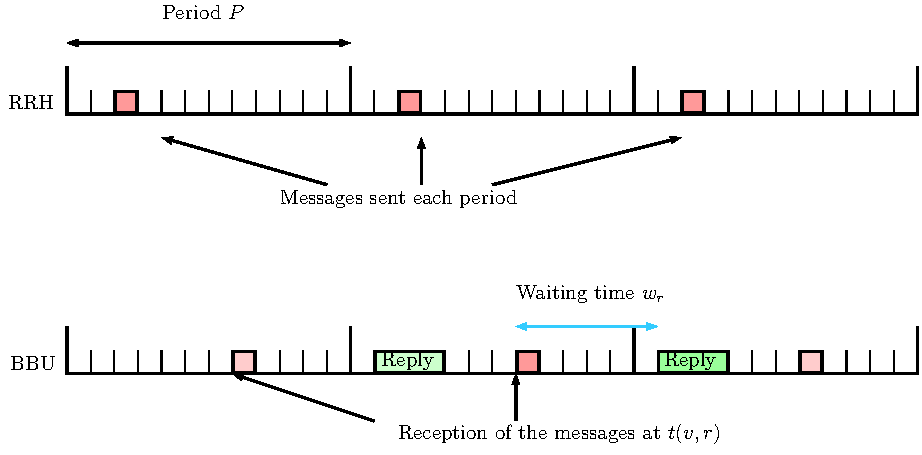
\includegraphics[width=0.9\textwidth]{rrh.pdf}
      \end{center}
      \caption{The process defined by a $P$-periodic assignment}
      \end{figure}

The process time for a message sent on the route $r$ is equal to $PT(r)=\lambda(r)+ w_r+\lambda(r)$. Each route must respect some time limit that we call a \emph{deadline}. To represent these deadlines, 
      we use a deadline function $d$, which maps to each route $r$ an integer such that $PT(r)$ must be less than $d(r)$.
    We can now define a first problem:

      \noindent {\bf Periodic Assignment for Low Latency (\pall)} 

 
      \noindent {\bf Input:}  A symmetric routed network $(G,{\cal R})$, the integers $P$ and a deadline function $d$.
      
      \noindent {\bf Question:} does there exist a $P$-periodic assignment $m$ of $(G,{\cal R})$ such that for all $r \in {\cal R}$, $PT(r) \leq d(r)$?

It turns out that the problem \pall is $\NP$-hard to solve and even to approximate for \emph{general} routed networks, and for the simplified version presented here~\cite{latency2017}.      
          
  \subsection{N-GREEN Optical ring}
  In this paper, we consider $G$ as a circular digraph $C_N$ representing an unidirectional optical ring. The vertices of the graph represents the nodes of the ring. In our study, we want to focus on the ring only. Thus, we ignore the external network and we consider that, the first and last vertex , $u$ and $v$ of the routes are some nodes of the ring. We consider a symmetric routed network. For each forward route $r$, the backward route $\rho(r)$ is the other part of the ring. Consequently, for each route $r$, $\lambda(r) + \lambda(\rho(r)) = RS$, where $RS$ is the size of the ring. In our experiments, we consider only one datacenter into the ring. This mean that all the forward routes have the same destination nodes, and all the backward routes have the same source node.

  The ring follows a broadcast and select behavior. When a packet is inserted in a slot on the ring, by a node, no other nodes are able to write on this slot. This packets can contain some data from several nodes on the ring, that are able to read in the packet. The only node which has the right to remove the packet from the slot is the owner. This mean that every packet makes exactly one lap of the ring. Furthermore, to write on a slot, a node has to have an empty slot in it's writing slot.
 \subsection{Message Granularity}
 Each arc $(u,v)$ can be represented as a sequence of slots $\{s_1, ... , s_k\}$, with $k = \omega(u,v)$. We denote by $s_n(u,v)$ the $n^{th}$ slot of the arc $(u,v)$. $s_i(v), i\in \{-\omega(u,v), ... , -1\} \cup \{1 , ... , \omega(v,w)\}$ is the $i^{th}$ slot after (before if $i<0$) v on the ring.
    On the following example, the red slot can be denoted by $s_2(u,v)$, $s_2(u)$ or $s_{-6}(v)$. 
    \begin{figure}[h]
    \centering
      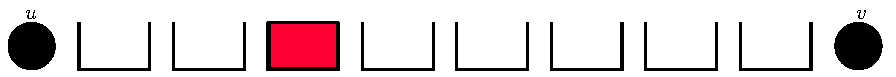
\includegraphics[scale=0.5]{suv.pdf}

      \caption{A link $(u,v)$ represented as a sequence of slots}
  \end{figure}
  
  Each node $v$ has a reading access on $s_{-1}(v)$ and a writing access on $s_{1}(v)$. Those slots are named respectively the reading and writing slots of $v$. Thus, during a time slot, a node $v$ can insert a {\bf container} on it's writing slot, if it is allowed to. At the end of the time slot, each packets rotate to the next slot. A packet emitted by a node $u$ on it's writing slot $s_1(u)$ will be available in reading for a node $v$ on it's reading slot, $s_{-1}(v)$, $d(u,v) -1$  time slots later.
\begin{figure}[h!]
      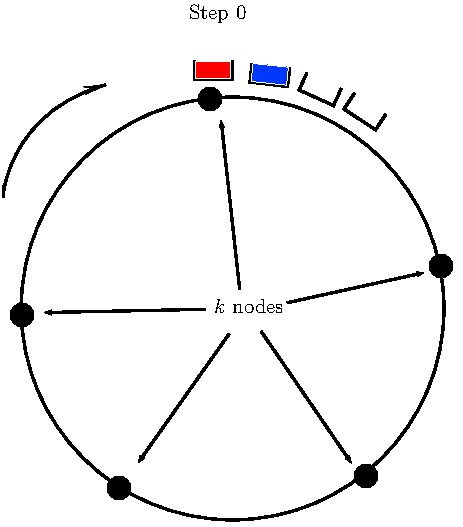
\includegraphics[scale=0.5]{anneau1.pdf}
      \hspace{3cm}
      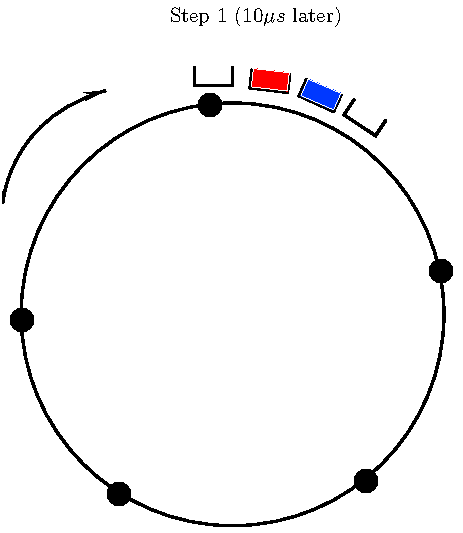
\includegraphics[scale=0.5]{anneau2.pdf}
      \caption{One rotation of the ring}
  \end{figure}

\subsection{Into the node : Two kind of traffics}
  In this study, we focus on the behavior of the N-GREEN optical ring. Therefore, we do not want to consider the problems caused by the upstream network. We model the arrival of messages in a node by the following way.
    To build the containers that are sent in the ring, a node has to deal with two kinds of traffic: 
    \begin{itemize}
    \item The {\bf Best effort traffic}, representing the internet flow.
    \item The {\bf C-RAN traffic}, with an higher priority than the best effort.
    \end{itemize}
    Let us denote {\bf BE-message} and {\bf CRAN-message} the unit of data of this flows. A container can be made of several BE-messages or CRAN-messages, and can be a combination of both kind of messages.

  \subsection{Messages arrival}
   To refine our model around the N-GREEN study, one must consider the following. The RRHs send some heavy packets in the network. Those packets are carried to the node of the right through an electronic link. The bandwidth of electronics networks is often smaller that opticals network bandwidths. An optical node on the ring is able to transform an electronic packet of size $x1$ measured in$\mu$s in an optical packet of size$x2 < x1$. In our study, $x1 = 10$ and $x2 = 1$. 
    
\begin{figure}[h!]
\begin{center}   

      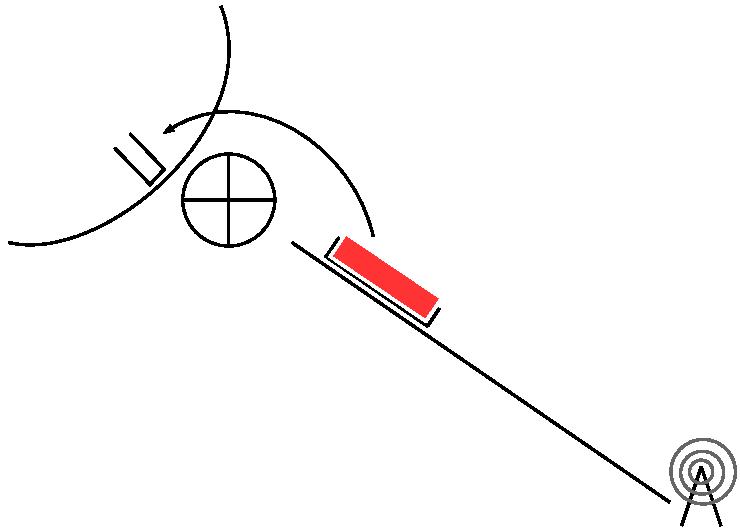
\includegraphics[scale=0.3]{slot1.pdf}
  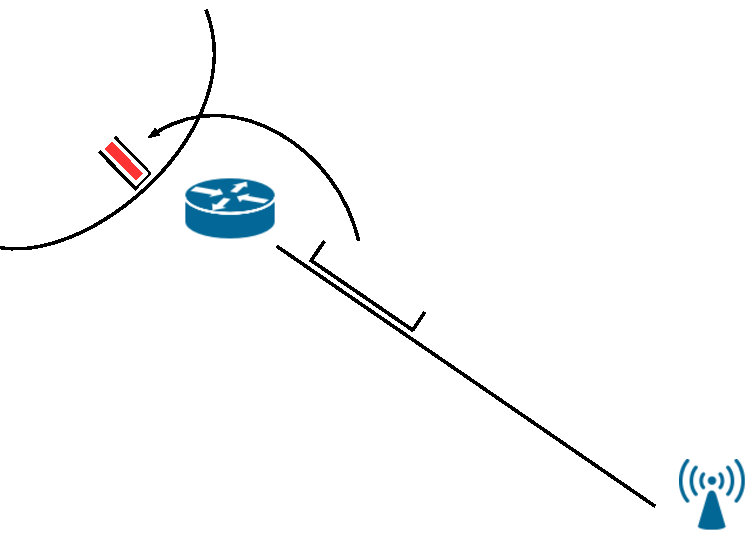
\includegraphics[scale=0.3]{slot2.pdf}
     \caption{Electronic-optical interface.}
     
\end{center}
  \end{figure}
  
   We want to look only at the optical ring, thus we consider that an RRH can send no more than a packet every $10\mu s$ on the ring. This gap between two messages from the same RRH is called $EP$, for {\bf Emission Period}.
    The messages of the RRHs cannot be transported in a single packet. We denote by $ET<P$,for {\bf Emission time}, the time during which an antenna emits a packet every $EP$ slots on the ring.An antenna emits $\frac{ET}{EP}$ packets on the ring, during a period $P$.
    	    
        \begin{figure}[h!]
\begin{center}   

      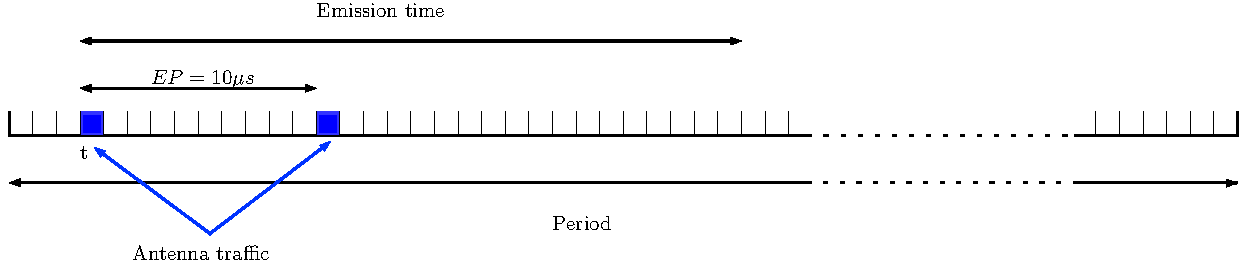
\includegraphics[width=\textwidth]{emission_antenna.pdf}
     \caption{Antenna traffic on the ring.}
\end{center}
  \end{figure}
  
  This specificity gives us a new problem, similar to \pall. The set of time slots used by route $r$ at vertex $v$ in a period $P$, is now defined by $[t(v,r)]_{P,EP} = \{t(v,r) +k \mod P \mid k \in \{0,EP,2\times EP,...., \frac{ET}{EP}\times EP\} \}$. Consequently, we now want to find a $(P,ET)$-periodic assignment that set the offsets of the routes $m_r$, such that there is no collision between two routes $r_1$ and $r_2$, that is, $[t(v,r_{1})]_{P,EP} \cap [t(v,r_{2})]_{P,EP} \neq \emptyset$. 
  The main purpose of this paper is to reduce as much as possible the latency of the C-RAN traffic, without increasing too much the latency of th BE traffic.
  \pall is a sub-problem of this problem with ET = 1. Thus, we can consider the complexity results for this problem too.
  \todo{pas sur d'avoir le droit de dire ca}

  
   \section{Performance evaluation of the N-GREEN optical ring}
   In a first time, we will look at the performance of the N-GREEN optical ring with an opportunistic insertion policy \cite{refngreen?}. When a node decides to send a container on the ring, it uses the first available slot in its writing slot.
    We study the performance through two messages management algorithms; a full opportunistic algorithm, and an algorithm that prioritize the C-RAN messages.
   For those two algorithms with opportunistic insertion policy, the offsets $m_r$ of the routes are chosen randomly in the period. 
   Since we do not manage those offsets, the two following algorithms do not gives us some $(P-ET)$-periodic assignment. No choices are made on the offsets and thus, two routes can collides. Furthermore, the generation of the BE traffic is given by the numerical analysis of sec~\ref{SECJMF}
   \todo{Expliquer rapidement sans s'eterniser.}
    
    \subsection{Full opportunistic algorithm}
    \label{sec:fullopport}
    We first want to look at a simple configuration in which we do not manage the messages (BE or CRAN) arriving into the nodes. At their arrival, the BE and C-RAN messages are buffered in the node, and a node send a container if : 
     \begin{itemize}
    \item The oldest message of the buffer has arrived on the buffer before $t - \alpha$, where $t$ is the actual time.
    \item The fill rate of the buffer is greater or equal than $\beta$.
    \end{itemize}
    Those parameters $\alpha$ and $\beta$ are fixed by the network specification.\todo{ref sur les traveaux de jmf et youssef}

    \begin{figure}[h!]
        \begin{center}
      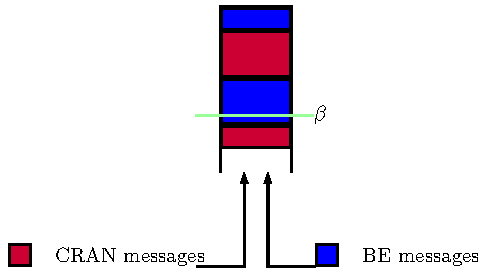
\includegraphics[scale=0.5]{insertionbuff.pdf}

      \caption{The packet creation buffer}
      \end{center}
  \end{figure}

This behavior is the basic one, the buffer of a node is filled following the FIFO rule by the BE and C-RAN messages. Then, when the node has an available free slot in its writing slot, the container is created and inserted in the slot if one of the previous constraints are satisfied. Otherwise the node does not send anything.

The following experiment shows us the performance this {\bf full opportunistic} algorithm with some parameters issued from N-GREEN. The optical link has a data flow of $100$Gbps, while a slots has a duration of $1\mu$s. The length of the ring is to $20$km in our simulations, this means that the ring has a length of $RS = 100$ slots. We denote {\bf latency} of a message the amount of time time the message has waited between its arrival in the node and its sending on the ring. On fig~\ref{fig:oport}, one can see the cumulative distribution latency of the different kinds of traffics on the ring. We chose to distinguish the traffic of the datacenter to the rest of the traffic, because the datacenter has a different behavior compared to the rest of the nodes. Those results are computed on $100$ instances of optical rings that have run during $10,000$ slots. We consider some BE messages of $125$B, and we configured the random generator such that each node load the network with an average of $5\%$ of BE traffic. We set $ET = 500$ slots and $EP = 10$ slotsn that correspond to respectively a C-RAN traffic of $5$Gbps and some electronic links of $10$Gbps data flow.The period  $P$ is to $1$ms, that is $1000$ slots. We set the number of antennas to $n=5$. We take $5$ nodes and one of them is the datacenter. The antennas are apportioned between the others node. With those parameters, the network is theoretically loaded to $75\%$. We set the parameters $\alpha = 10 \mu$s and $\beta = 0.7$, following the numerical analysis (see~\ref{sec:JMF}). 

We chose to distinguish the different traffics; The uplink traffic is the C-RAN traffic going from the RRHs to the BBUs. The downlink traffic corresponds to the messages going from the BBUs to the RRHs. We also make a difference between the BE messages on the nodes connected to some RRHs (BE) with the BE messages coming from the datacenter(BBU BE). In this case, this is not relevant, but some future experiments will reveal a difference between those two kind of BE traffics.
    \begin{figure}[h!]
    \label{fig:oport}
        \begin{center}
      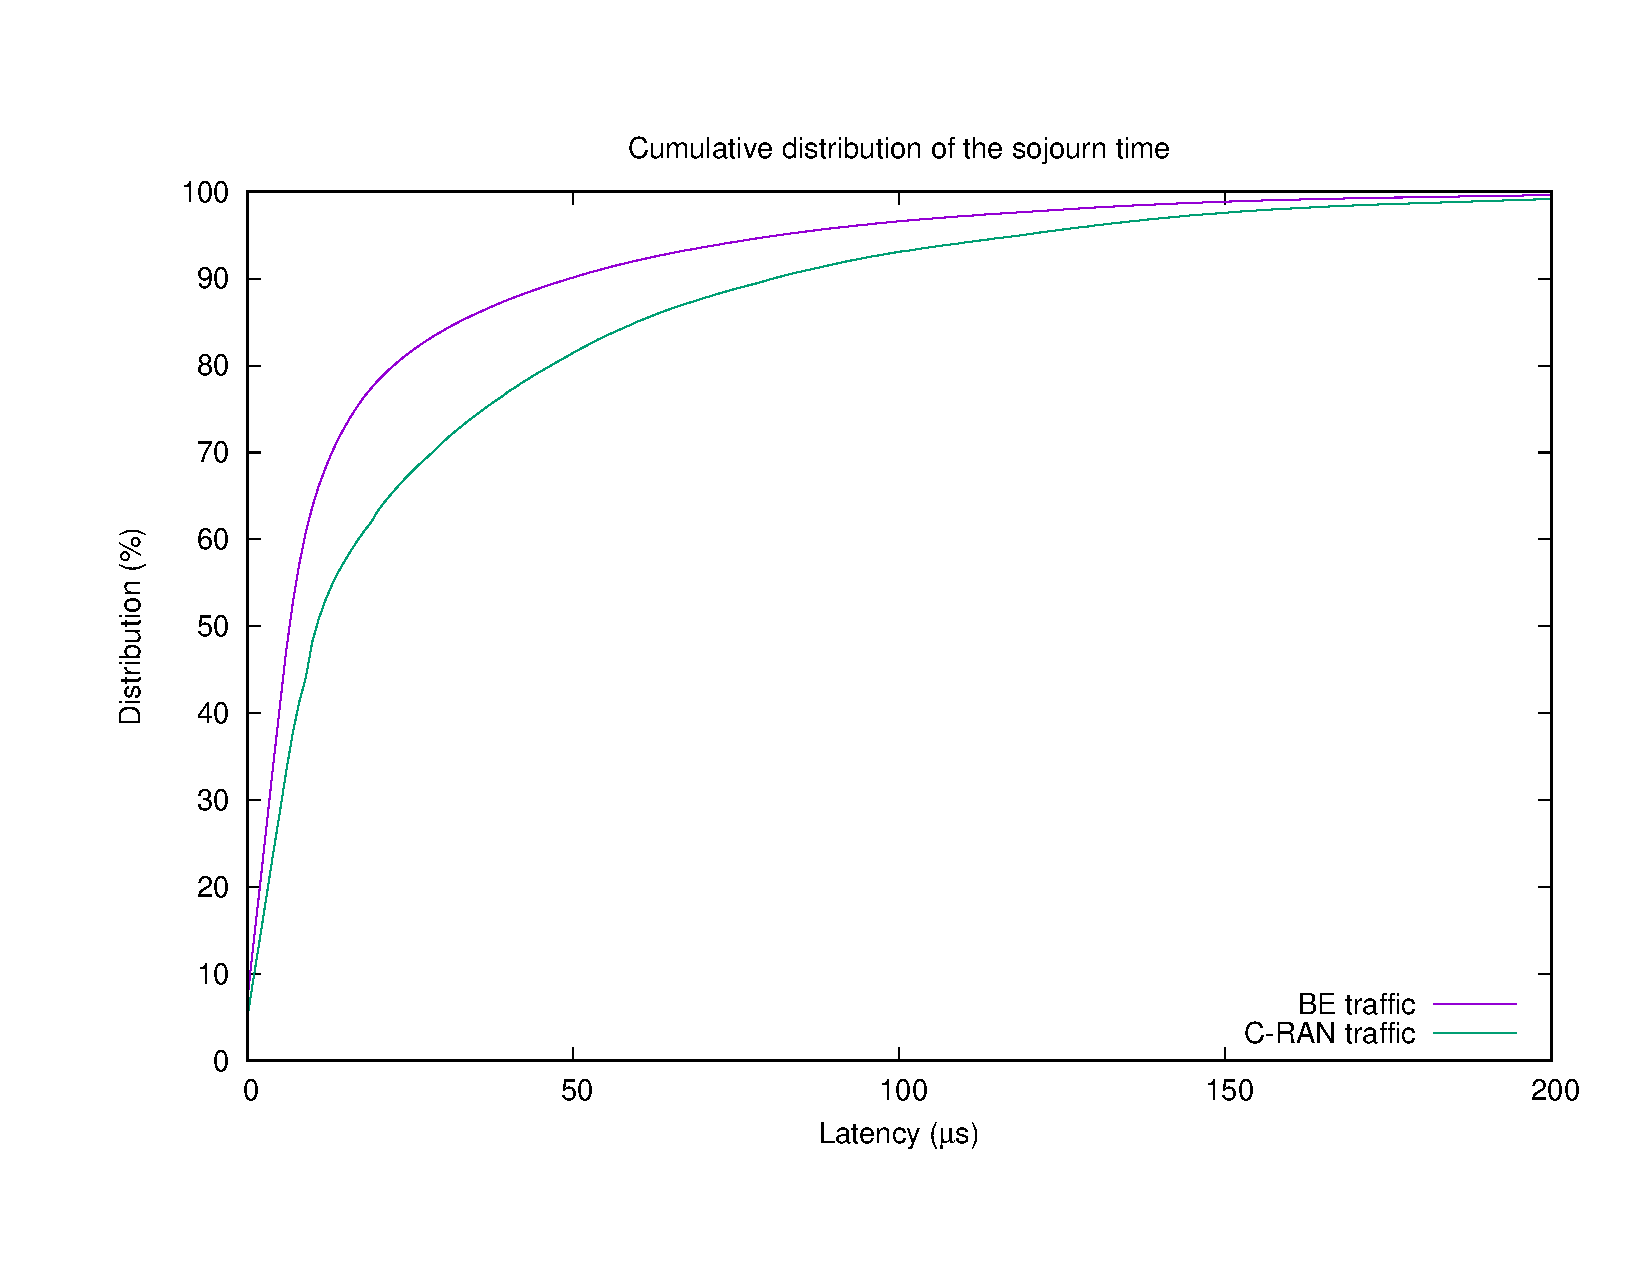
\includegraphics[scale=0.4]{oport}

      \caption{Full opportunistic algorithm performances.}
      \end{center}
  \end{figure}
  
  As we can see on fig~\ref{fig:oport}, the latency for the different kind of traffic is notably similar because we do not manage anything. Furthermore, we can remark that about $20\%$ of the C-RAN messages wait over $200$ms, that is the maximum latency allowed for C-RAN \cite{REF}.

\subsection{C-RAN priority algorithm}
  In order to improve the C-RAN-messages latency, we imagined the following solution. Each nodes have two buffers. One for the BE messages, and one fore the C-RAN messages. When a node is able to send a container on the ring, i.e. the slot on it's writing slot is free, the container is filled with the C-RAN messages first. The buffer that contains the C-RAN messages does not take into account the parameters $\alpha$ and $\beta$ we described in sec~\ref{sec:fullopport}. If there is some C-RAN messages in the buffer, we send it, even if the container is not full enough. Nevertheless, in this situation, the nodes always tries to fill the container with some BE messages. If there is no C-RAN messages in the buffer, the node have the same behavior as in the full opportunistic algorithm. We call this algorithm the {\bf C-RAN priority algorithm}.
  
    \begin{figure}[h]
\begin{center}   
      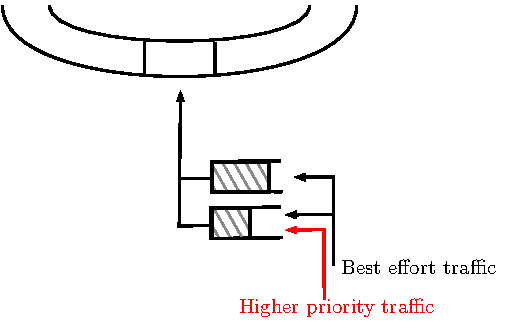
\includegraphics[scale=0.7]{insertion1.pdf}
     \caption{C-RAN priority buffer.}
\end{center}
  \end{figure}
  
  With this algorithm, one can imagine highly improve the latency of the C-RAN messages. Fig~\ref{fig:prior} shows us the performance of the C-RAN priority algorithm for different kinds of traffics. The parameters of the simulations are exactly the same as those of the previous experiment.
  
      \begin{figure}[h]
      \label{fig:prior}
\begin{center}   

      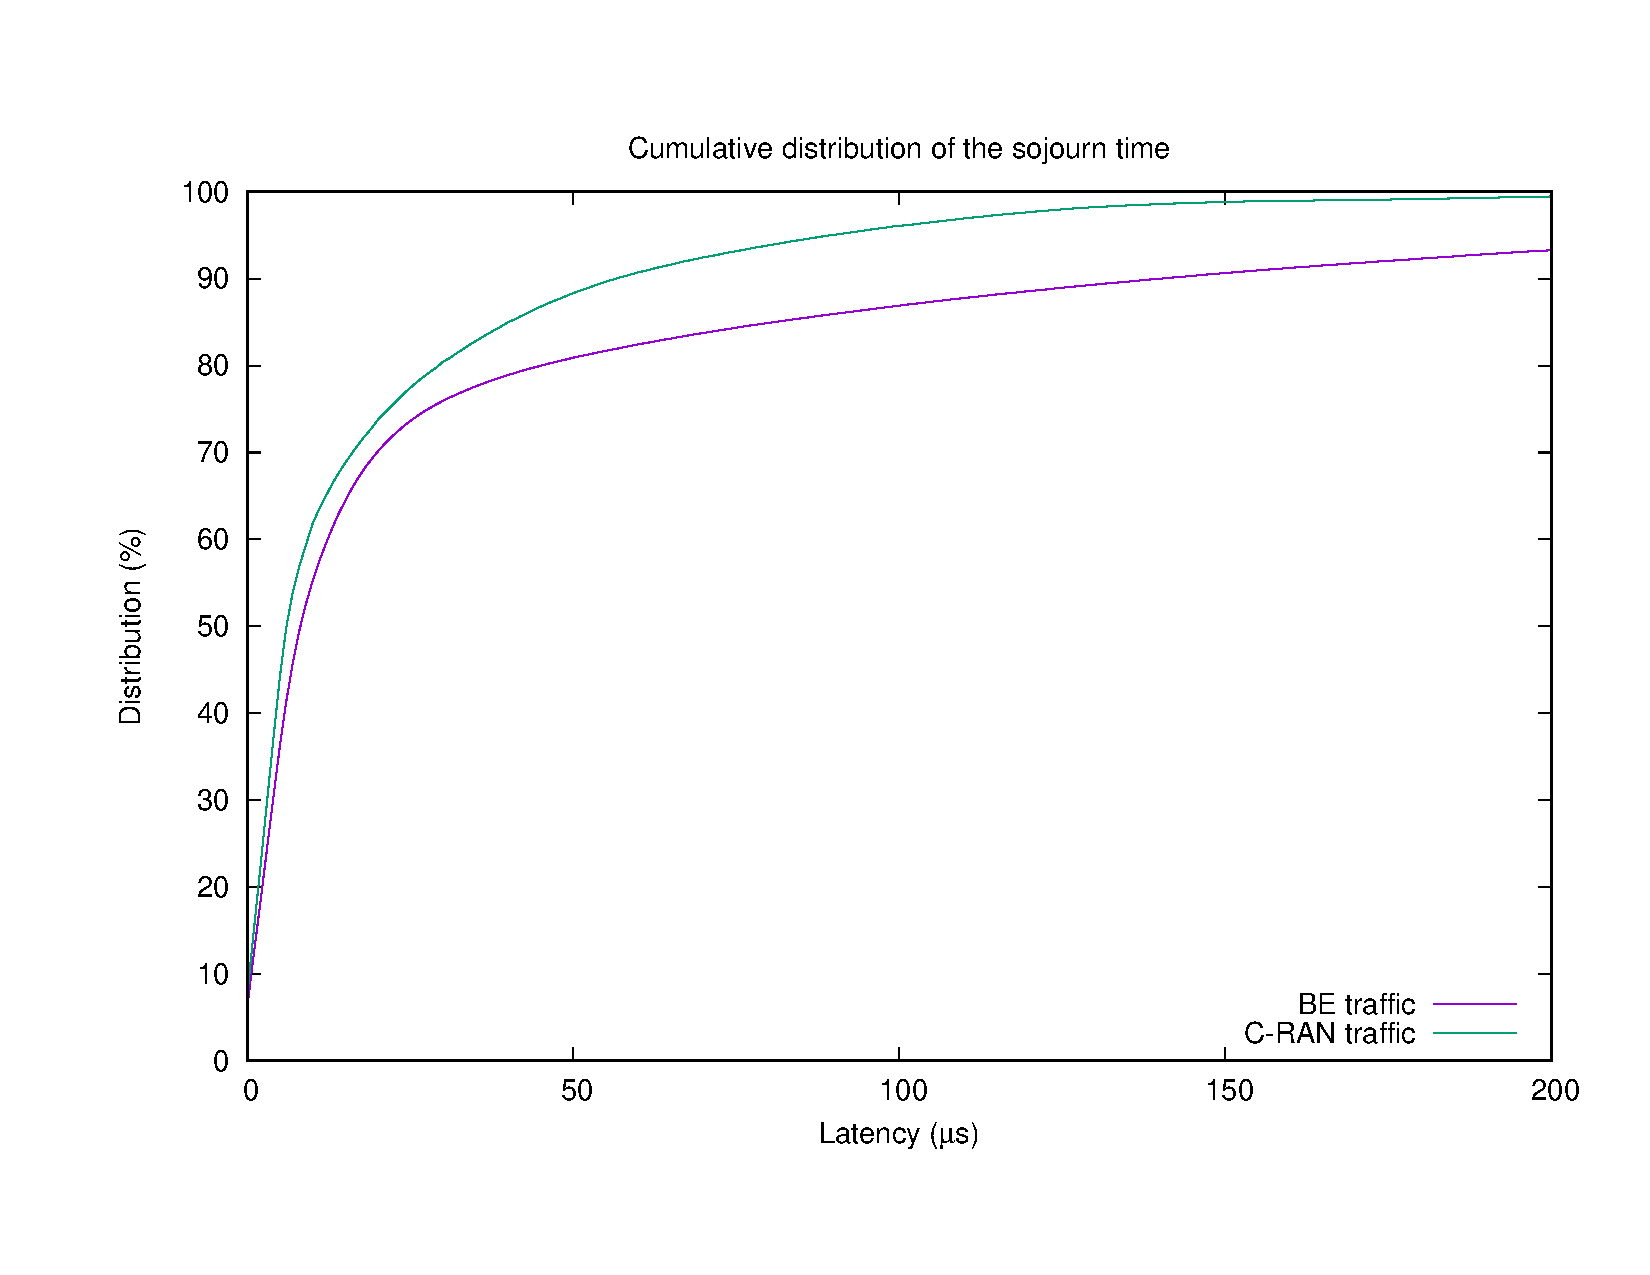
\includegraphics[scale=0.4]{prior.pdf}

     \caption{C-RAN priority algorithm performances.}
\end{center}
  \end{figure}
  
  As expected, the latency of the C-RAN messages is highly decreased compared to the full opportunistic algorithm. Nevertheless, there is still $5\%$ of the downlink messages that have more than $200 \mu$s of latency, and the best effort are highly penalized.
  \todo{il manque une partie sur le travail de karim, au moins pour le deliverable}
  Thus, we propose a deterministic approach in which we set the offsets of the antennas and we reserve the slots needed for the containers with the CRAN messages. For the rest of the section, the policy of slot insertion is the slot reservation. \todo{pour l'article, ne pas mettre}
  
  \section{Deterministic approach for 0 latency on C-RAN}
\label{det}
\subsection{Slot Reservation}
To decrease the C-RAN messages latency, one plan to reserve the slots for the nodes. Indeed, if a nodes $i$ needs to send a container in its wrtting\_slot at time $t$, this slot needs to be reserved during the previous lap of the slot, i.e. at time $t - RS$ by $i$. In this situation, if the slot is already taken by a packet which has been sent by a node $k$, $k$ will remove the packet of the slot during the next lap of the ring, and no other nodes are able to write in this slot before it comes back to the node $i$ a date $t$. By finding a $(P,ET)$-periodic assignment and reserving the corresponding slot, we allow the C-RAN messages to have $0$ latency in nodes. Though, it impacts the best effort, by avoiding them to use free reserved slots. It is equivalent to increase the load of the network, without increasing the number of messages carried by the network. 

In this section, we explain the different algorithm we use to have $0$ latency on C-RAN messages and we study their impact on the BE messages latency.
  
Unlike the previous algorithms with opportunistic insertion policy, we now want to choose a $(P,ET)$-periodic assignment for the routed network $(G,{\cal R})$. An antenna can not emit a message more often than one slot every $EP$ slots. We define a {\bf macro slot} as a duration of $EP$ slots, in which each antenna can emit at most once. Since all the forward routes have the same last vertex $v$ (the datacenter), which is also the first vertex of all the backward routes, we choose to look at the behavior of the messages in this vertex only. The purpose is to determine $t(v,r_i)$ for each routes $i$, such that there is no collisions between the routes. Once $t(v,r_i)$ is set, it is easy to compute $m_{r_i} = t(v,r_i) - \lambda(v,r_i)$.

\subsection{N-GREEN parameters adapted algorithms}
An antenna cannot emit more than once every macro slot, thus, we consider the simple case in which there is less antennas than slots in a macro slot. Since a BBU emits an answer to it's RRH, for each antennas, two slots must be reserved. Thus, we first study the case $EP \ge 2\times n$. 

 In this section, the algorithms assign two slots to each antenna: one slot for the uplink and one slot for the downlink traffic in the macro slot. Since The BBU always send an answer to the RRH, one must consider that the BBU immediately send an answer after receiving a message from an RRH. This simplification allows us to reserve a set of two slots for each antennas. Let us call {\bf frequency} a set of two slots in a macro slot. The purpose is then to assign to each antenna a frequency.
 
 Because there is at most as much couples BBU-RRH as frequencies, we want to assign one antenna to one frequency.
We propose the following {\bf naive reservation algorithm}. For each antenna on the route $i, i\in [0;n-1] $, set $t(v,r_i)= 2\times i$ with $v$ the vertex of the BBUs. 
   \begin{figure}[h]

      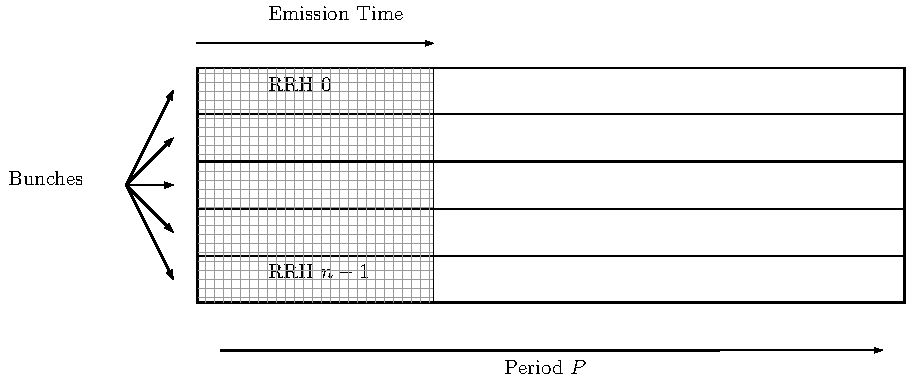
\includegraphics[scale=0.7]{freqgrouped.pdf}
     \caption{Grouped assignment of the frequencies to the antennas.}   \label{fig:freqG}
  \end{figure}


We kept the same parameters than in the two previous experiments and we made an experiment to show the impact of this algorithm on the BE traffic. Fig~\ref{fig:res1} shows us the performance of this algorithm for different kinds of traffics. 

      \begin{figure}[h]
\centering
      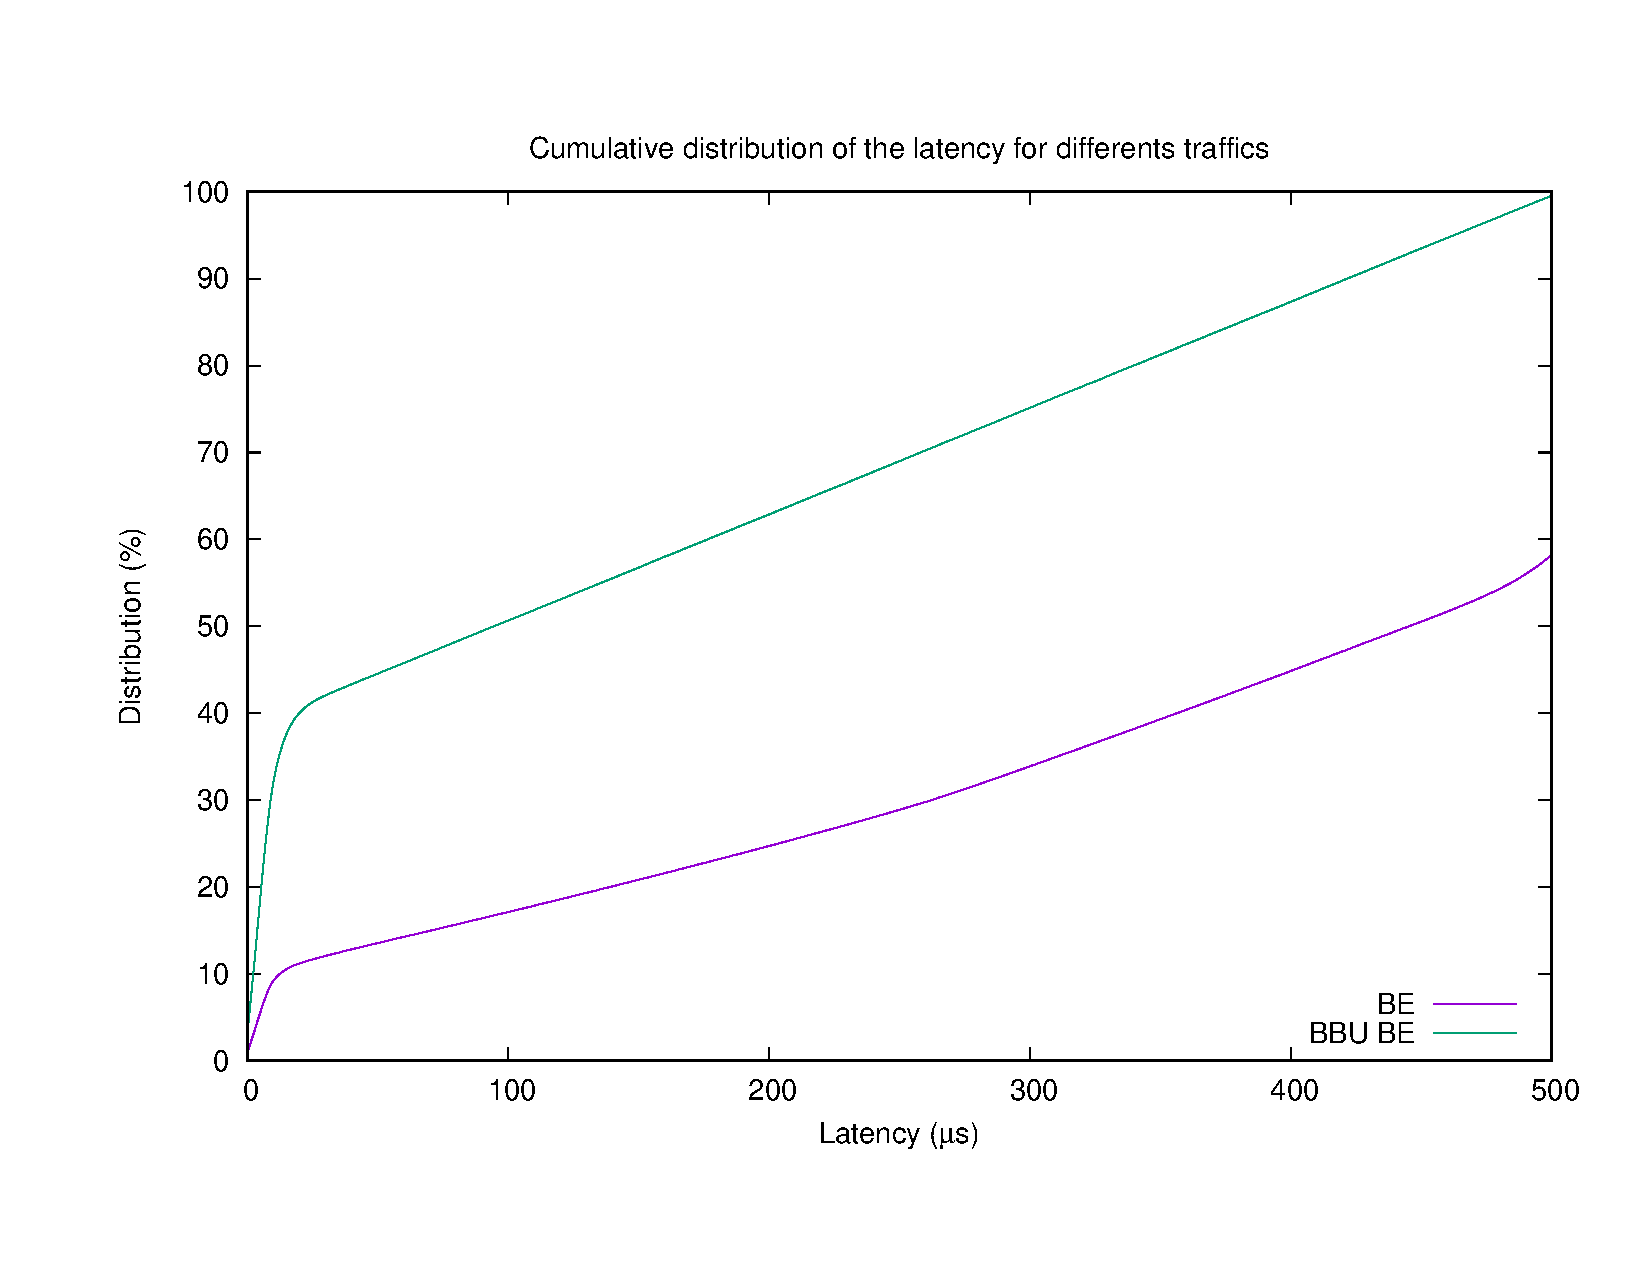
\includegraphics[scale=0.4]{res1.pdf}
     \caption{Impact of the naive reservation algorithm on the Best effort flows.}   \label{fig:res1}
  \end{figure}

As we can see, the BE traffic is highly penalized by this algorithm, indeed, while almost $100\%$ of the BE messages have a latency to less than $300 \mu$s with the full opportunistic algorithm (see fig~\ref{fig:oport}), here, the BE messages coming from the datacenter can be buffered up to $500\mu s$, while half the BE messages of the others node have to wait more in the node before being sent in the ring. Those performances are explained by the structure of the algorithm. The messages are grouped together, and with our parameters, $EP = 2\times n$. It creates a long sequence of slots during which there is no free slots in the ring. This explain why half of the BE messages of the datacenter have an acceptable latency, while the other part have up to $500\mu s$ of latency.

There is another remarkable behavior on this experiment. The BE messages coming from the nodes with the RRHs have a significantly worst latency than the BE messages coming from the datacenter. Indeed, once a node is the owner of a slot, it is the only one that can remove the container from the slot. Also, the slot is freed in the reading slot of a node, and can immediately be re-used by the same node in it's writing slot. The period is split in two steps : one in which only there is only CRAN messages in the ring, and one in which the BE traffic can uses the ring. During the first step, the datacenter uses half of the slots for its CRAN traffic. That is why the datacenter can send close to $5$ times more messages than the others node.


To improve the BE latency, we propose then to balance the load of the CRAN traffic over the period. Instead of giving the same $t(v,r_i)$ for all routes $i$, with $v$ the datacenter, we now uniformly reppart the different $t(v,r_i)$ in the period. 
\todo{donner un nom a $t(v,r_i)$}

   \begin{figure}[!h]

      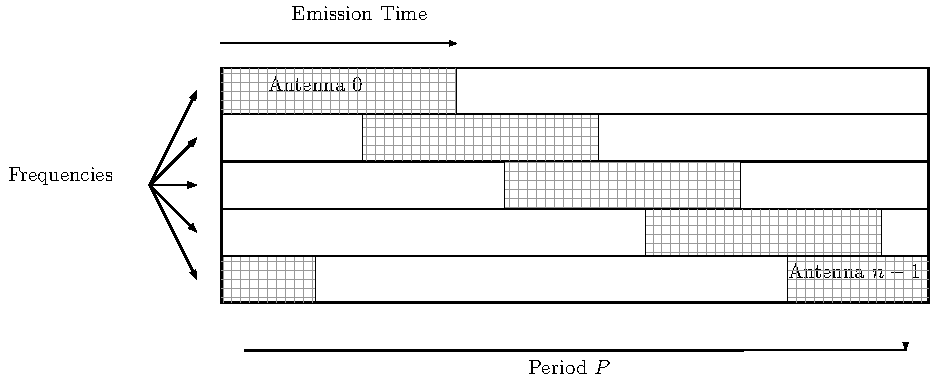
\includegraphics[scale=0.7]{freqsplited.pdf}
     \caption{Splited assignment of the frequencies to the antennas.}   \label{fig:freqS}
  \end{figure}
  
  With this algorithm, the load of the CRAN traffic is uniformly distributed on the period. There is no more the two steps phenomenon observed with the previous algorithm. On fig~\ref{fig:res2} on can observe the performance of this algorithm on the best effort. Once again, to have a reference point, we take the same parameters for the simulation.

 \begin{figure}[h]
\centering
      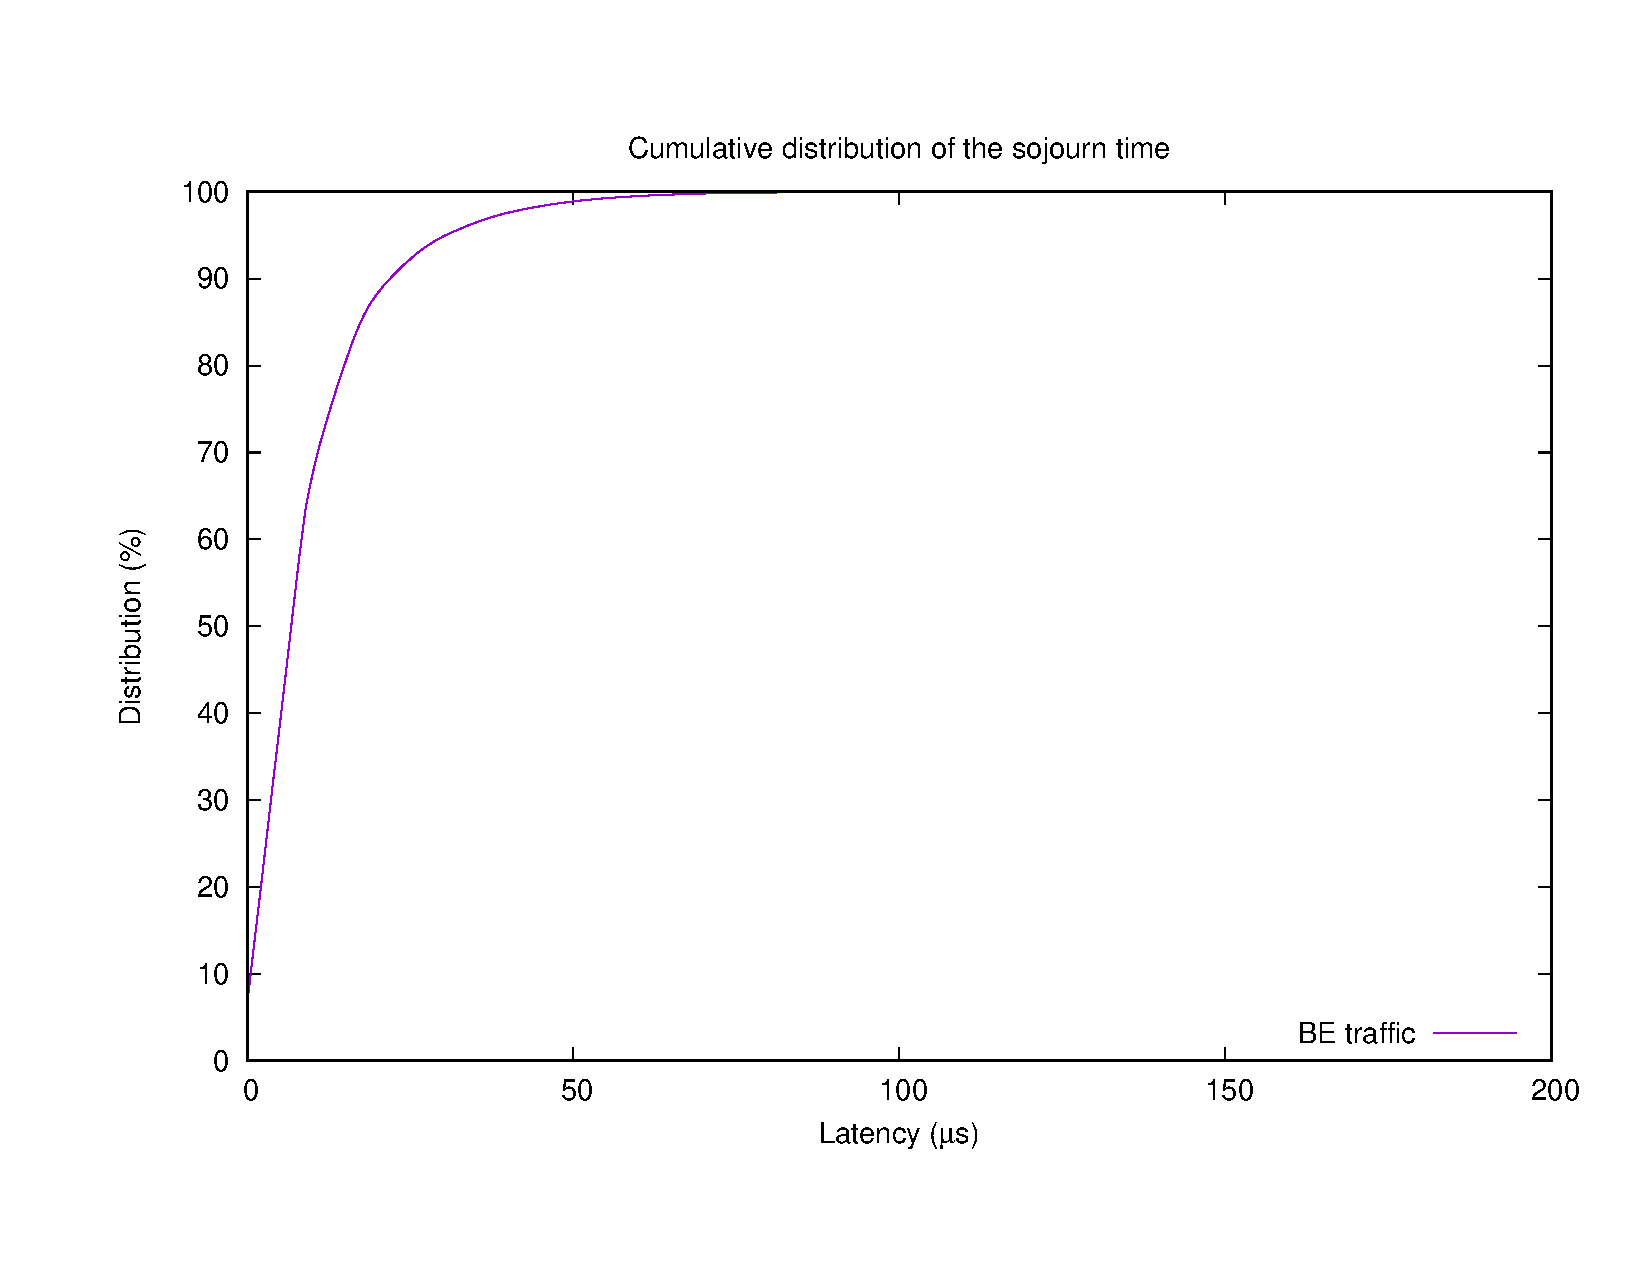
\includegraphics[scale=0.4]{res2.pdf}
     \caption{Impact of the splited reservation algorithm on the Best effort flows.}   \label{fig:res2}
  \end{figure}
  
  As we can see, the latency of the BE messages is highly better with this this algorithm. Nevertheless, there is still a lack of balancing between the messages coming from the datacenter and the messages coming from the RRH nodes. Indeed, the latency of the BBU BE is always less than $100 \mu s$, which is better than the full opportunistic algorithm, while almost $20\%$ of the others BE have a latency greater than $500\mu s$, which is worse than the full opportunistic algorithm. Thus, we decreased the latency of every kind of traffic but the BE coming from the RRH, which are, the major part of the BE messages. One can imagine a policy that manage the load of the BE traffic on the datacenter, but it is out of our study which focus on CRAN performances.

\subsection{With more antennas}
 In this section, we study the case $n > \frac{EP}{2}$. Indeed, if we want to assign more than one antenna to a frequency. 
 Let us consider a particular behavior of the ring. Instinctively, we can think that if we have enough space in the period for many traffics on the same frequency that is, $ET \le \frac{P}{2}$, we can assign several antennas to the same frequency, i.e. $n > \frac{EP}{2}$. In fact, this is not always possible. 
 \begin{prop}
If $ET = \frac{P}{2}$, there is no $(P,ET)$-periodic assignment if $n > \frac{EP}{2}$.
 \end{prop}
 \begin{proof}
 Let us take $ET =  \frac{P}{2}$ and $n = \frac{EP}{2} + 1$. We assign a frequency to each $EP$ first antennas and we have only one antenna left. Then, we can look at only one frequency. 
 
 We take a ring with two nodes $A$ and $B$. We look at the behavior of one frequency, thus, both the nodes emits some packets every slots, during $ET$ slots. By construction, we allow $A$ to emit a time $1$ during $ET$ slots. This messages arrives in $B$ at $\omega(A,B)$, that is  $[t(B,r_A)]_{P,EP} = [\omega(A,B);\omega(A,B)+ET]$. Then, $B$ can imedialty emit its message at time $\omega(A,B)+ET$. This messages from $B$ arrives at $A$ at time $\omega(A,B)+ET + \omega(B,A) = ET + RS$, and thus, $[t(A,r_B)]_{P,EP} = [ET + RS;ET + RS + ET] = [ET+RS; RS + P] = [ET + RS; RS] \mod P$. Since $[t(A,r_A)]_{P,EP} = [1;ET]$, there is a collision between the two routes $A$ and $B$.
  \begin{figure}[h]
\centering
      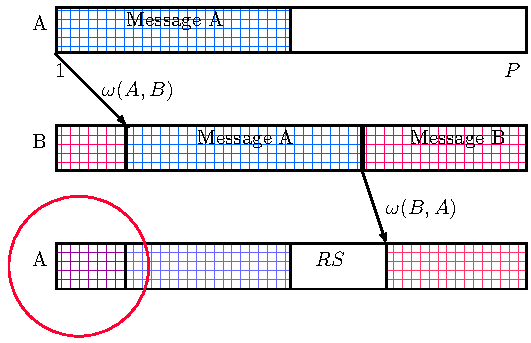
\includegraphics[scale=0.7]{rs.pdf}
     \caption{Collision between two routes on the same frequency when the period is too small.}   \label{fig:proofrs}
  \end{figure}
 \end{proof}
 
 
 As we have just noted, if several antennas share the same frequency, the period must have an additional budget in addition to the time needed to send the messages. Let us study the size of the additional budget.
 \begin{prop}
 If several antennas shares a frequency, one might have $P = n\times ET + RS$ , with $a$ the number of antennas.
 \end{prop}
 \begin{proof}
 We seek to show that proposition by induction.
 
 {\bf Base case:} For $n = 2$, the proof of the previous example shows us that it is possible to assign two routes on the same frequency with $P = 2\times ET + RS$.
 
 {\bf Induction step:}  We consider that we have a frequency shared by $n$ antennas, with a period of size $P= n\times ET + RS$. We want to show that if we want to add one antenna to the frequency, we need a period of size at least $P = (n+1)\times ET + RS$. If we look at the sequence period of the frequency with $n$ antennas, we can observe that this sequence is the same in every nodes, shifted of the length of the routes between two nodes. For instance, if we take two nodes $A$ and $B$, the sequence in $A$ is the same that the sequence in $B$ shifted of $\omega(A,B)$.
 
   \begin{figure}[h]
\centering
      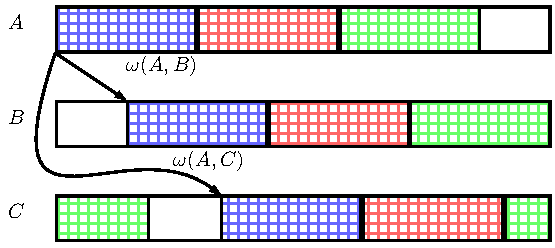
\includegraphics[scale=0.7]{period1.pdf}
     \caption{An example of sequence with n = 3.}   \label{fig:proofperiod1}
  \end{figure}
   
 Thus, if we add $ET$ slots in this frequency, the periodic emissions of all others nodes are not impacted, there is just a new interval in the sequence.
 
   \begin{figure}[h]
\centering
      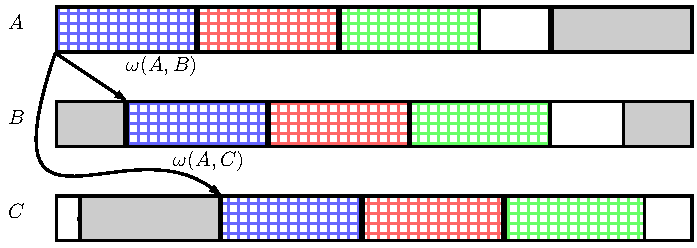
\includegraphics[scale=0.7]{period2.pdf}
     \caption{The same sequence with n = 4.}   \label{fig:proofperiod2}
  \end{figure}
  Note that a node can send some traffic from more than one antenna, the figures ~\ref{fig:proofperiod1} and \~ref{fig:proofperiod2} are just an example, but this proof stays the same.
 \end{proof}
 
Considering those results, we propose an algorithm to allow several antennas to share the same frequency, as long as $P = n\times ET + RS$. 
We first compute the number of frequencies needed to carry the number of antennas $n$. Then, the algorithms tries to balance those frequencies in all existing ones, i.e. it avoids to group the used frequencies in a macro slot.

The used frequencies have $RS$ or more free slots that the BE traffic can fill. Thus, the algorithm subsequently balance the first time at which a frequency have some CRAN, with the same idea than the splited algorithm.

   \begin{figure}[h]
\centering
      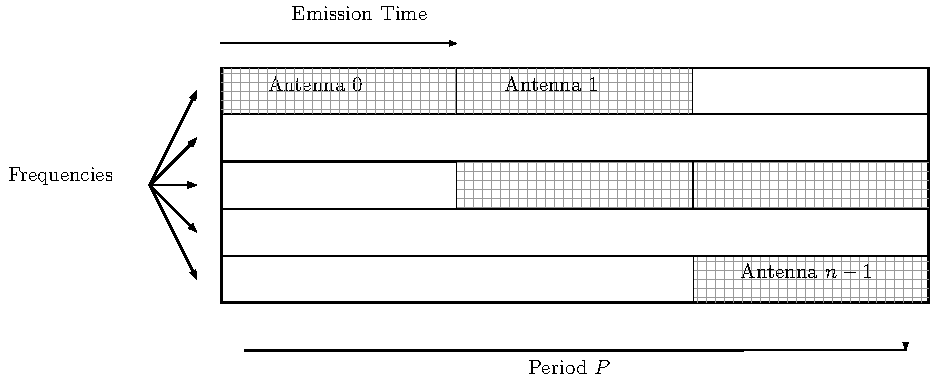
\includegraphics[scale=0.7]{optimalgo.pdf}
     \caption{Organization of the frequencies with the balancing algorithm.}   \label{fig:optimalgo}
  \end{figure}
  
  We want to observe the impact of this algorithm on BE traffics. Since our previous parameters did not allow several antennas to share a frequency, we now set $ET = 100$, that correspond to a C-RAN flow of $1$Gbps. This is not out of context since the exact split of the C-RAN is not fully determined yet~\cite{REF}. To keep a load similar to the load in the previous experiment, we set the number of antennas to $n=25$. The others parameters are all the one described in the first experiment.
  The following experiment shows us the impact of the balancing algorithm on the BE traffics.
  
   \begin{figure}[h]
\centering
      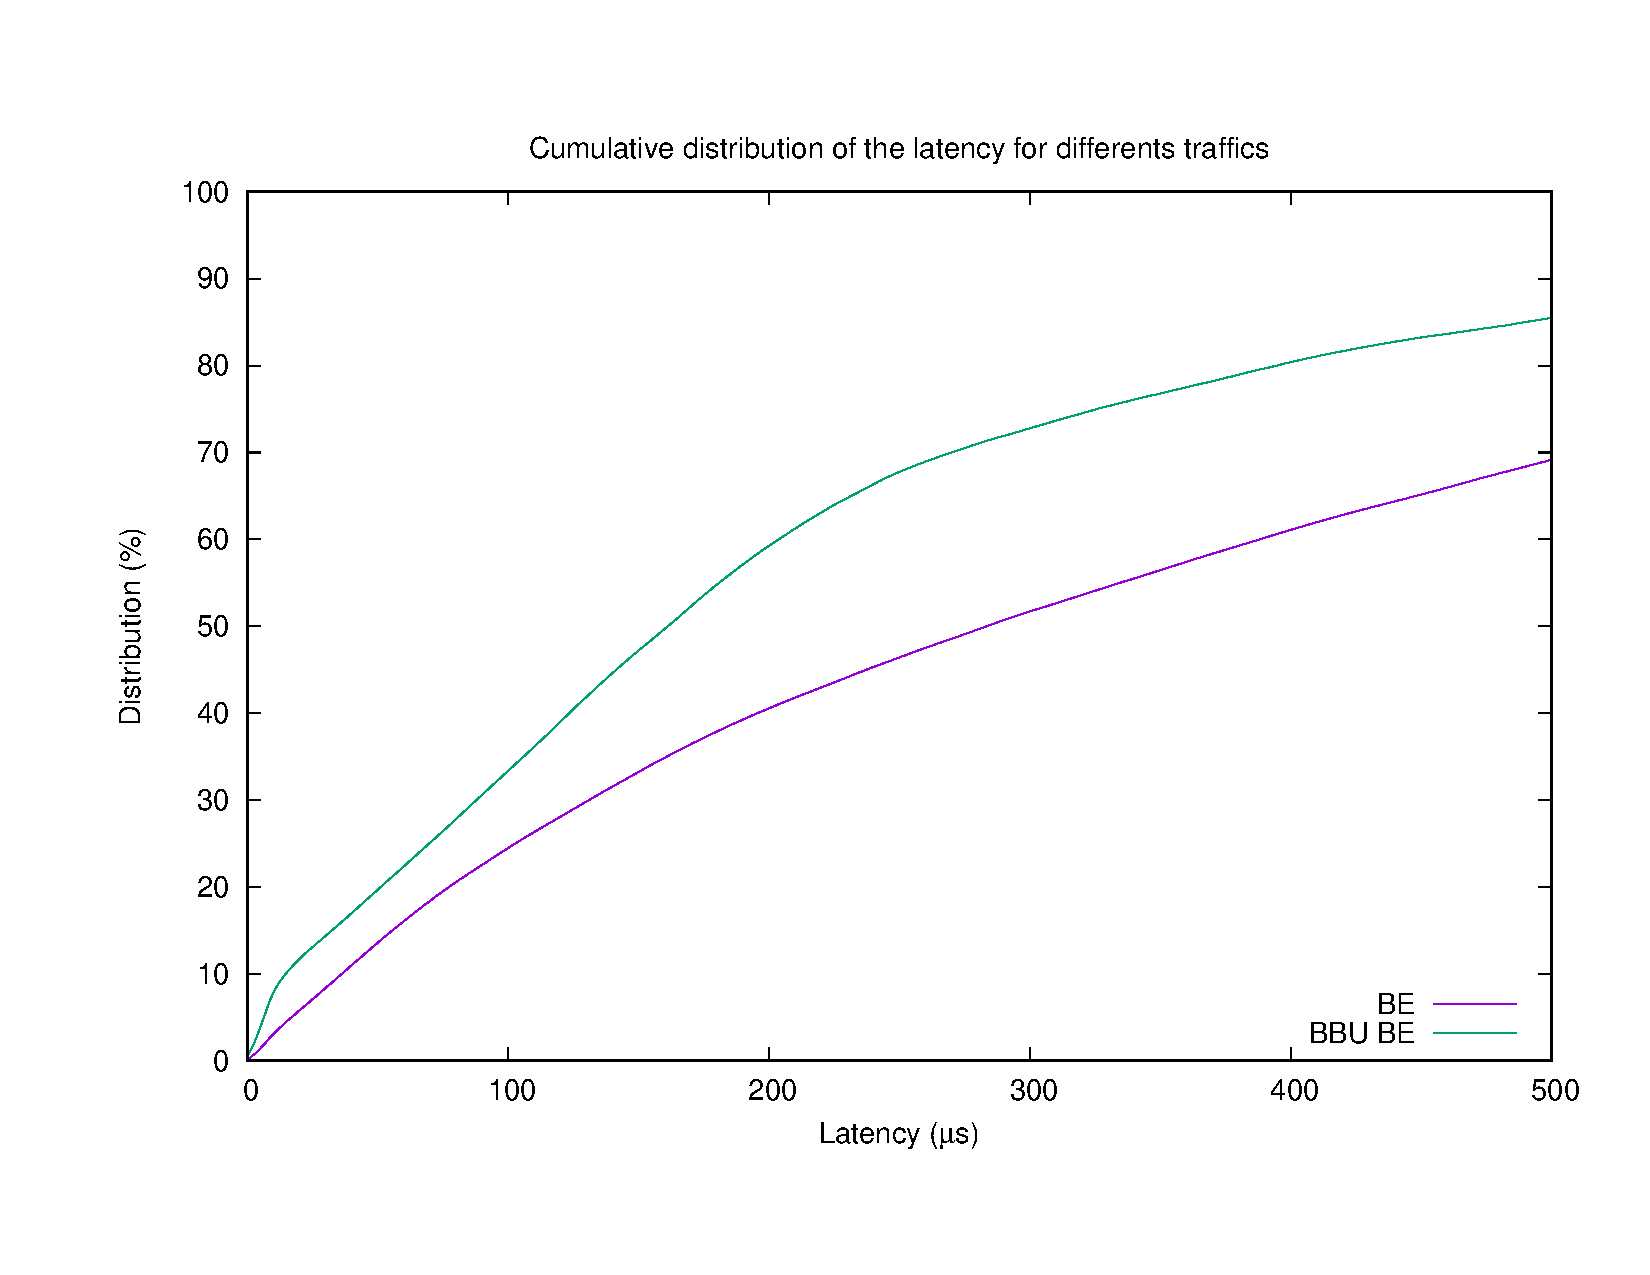
\includegraphics[scale=0.4]{opti.pdf}
     \caption{Balancing algorithm performance on the N-GREEN optical ring.}   \label{fig:optimres}
  \end{figure}
  
  As fig~\ref{fig:optimres} shows, the BE traffics are both impacted by this algorithm, but unlike the previous algorithm, it looks like there is a balancing between the BE of the BBU and the others BE. This behavior is probably due to the fact that there is less frequencies assigned to the BBU when there is some C-RAN in the ring. Indeed, since we tried to fill as much as possible the frequencies, and we kept the same load, we used less frequencies and thus, the BBU monopolize less resources than with the previous algorithms.
  
  \bibliographystyle{ieeetr}
\bibliography{src}

\end{document}